\documentclass[aps, prc, twocolumn, reprint]{revtex4-1}

\usepackage{amsmath}
\usepackage{mathtools}
\usepackage{amsfonts}
\usepackage{url}
\usepackage{xspace}
\usepackage{siunitx}
\usepackage[usenames,dvipsnames]{xcolor}
\usepackage{float}
\usepackage[caption=false]{subfig}
\usepackage{framed}

\frenchspacing

% Defined macros

\DeclareMathOperator{\csch}{csch}
\DeclareMathOperator{\sech}{sech}

\newcommand{\degree}[0]{\ensuremath{^\circ}\xspace}
\renewcommand{\implies}{\Rightarrow}
\newcommand{\eval}[1]{\ensuremath{\left<#1\right>}}
\newcommand{\ket}[1]{\ensuremath{\left| #1 \right>}}
\newcommand{\bra}[1]{\ensuremath{\left< #1 \right|}}
\newcommand{\mel}[3]{\ensuremath{\left<#1 \right|\! #2 \!\left| #3 \right>}}
\newcommand{\proj}[2]{\ensuremath{\left<#1 \middle| #2 \right>}}

\newcommand{\pmat}[1]{\ensuremath{\begin{pmatrix}#1\end{pmatrix}}}

\newcommand{\pder}[2]{\ensuremath{\frac{\partial #1}{\partial #2}}}
\newcommand{\ppder}[2]{\ensuremath{\frac{\partial^2 #1}{\partial #2^2}}}
\newcommand{\ppmder}[3]{\ensuremath{\frac{\partial^2 #1}{\partial #2 \partial #3}}}

\newcommand{\pderc}[3]{\ensuremath{\left( \frac{\partial #1}{\partial #2} \right)_{\!\!#3}}}
\newcommand{\ppmderc}[4]{\ensuremath{\left( \frac{\partial^2 #1}{\partial #2 \partial #3} \right)_{\!\!#4}}}

\newcommand{\nuc}[2]{${}^{#1}\text{#2}$}

\newcommand{\fresco}[0]{\textsc{Fresco}\xspace}
\newcommand{\sfresco}[0]{\textsc{Sfresco}\xspace}


\begin{document}

\title{PHY 982 Homework 2: Elastic scattering and optical models}
\author{Josh Bradt}
\author{Chris Izzo}
\date{April 9, 2015}

\maketitle

\section{Elastic scattering calculations}

	We chose to use the nucleus \nuc{100}{Mo} for our target. This nucleus has 42 protons and 58 neutrons. As an even-even nucleus, this target has a ground state of $0^+$.

	\subsection{Pure Coulomb potential}

	We began by running \fresco for elastic scattering of protons at \SI{5}{MeV} and \SI{50}{MeV}. We did this for a point-like potential with a Coulomb radius of \SI{0.001}{fm} and a finite potential with a Coulomb radius of \SI{1.220}{fm}. We chose the second value from the previous homework assignment. Fig.~\ref{fig:protons_nonuc} shows the differential cross sections of these reactions as a ratio to the Rutherford cross sections. We can see that the ratio to Rutherford is approximately 1.0 for all angles for the scattering off of the point-like potential. This is because a point-like potential produces pure Coulomb scattering. For the finite-radius potentials, we found that the ratio to Rutherford is still 1.0 for the low-energy scattering. This is because the low-energy proton does not penetrate beyond the Coulomb radius. The higher-energy proton, on the other hand, penetrates beyond the Coulomb radius and sees that the potential is different from charge concentrated at a point. This explains why the \SI{50}{MeV} proton scattering off of the finite potential produces a cross section that is different from Rutherford, while the others do not.

	Next, we repeated this analysis with neutrons instead of protons. This gave us the elastic scattering cross sections shown in Fig.~\ref{fig:neutrons_nonuc}. As we can see, the scattering cross section is very small. This is because the neutrons are neutral and shouldn't interact with the Coulomb potential. 

	\begin{figure}[bt]
		\centering
		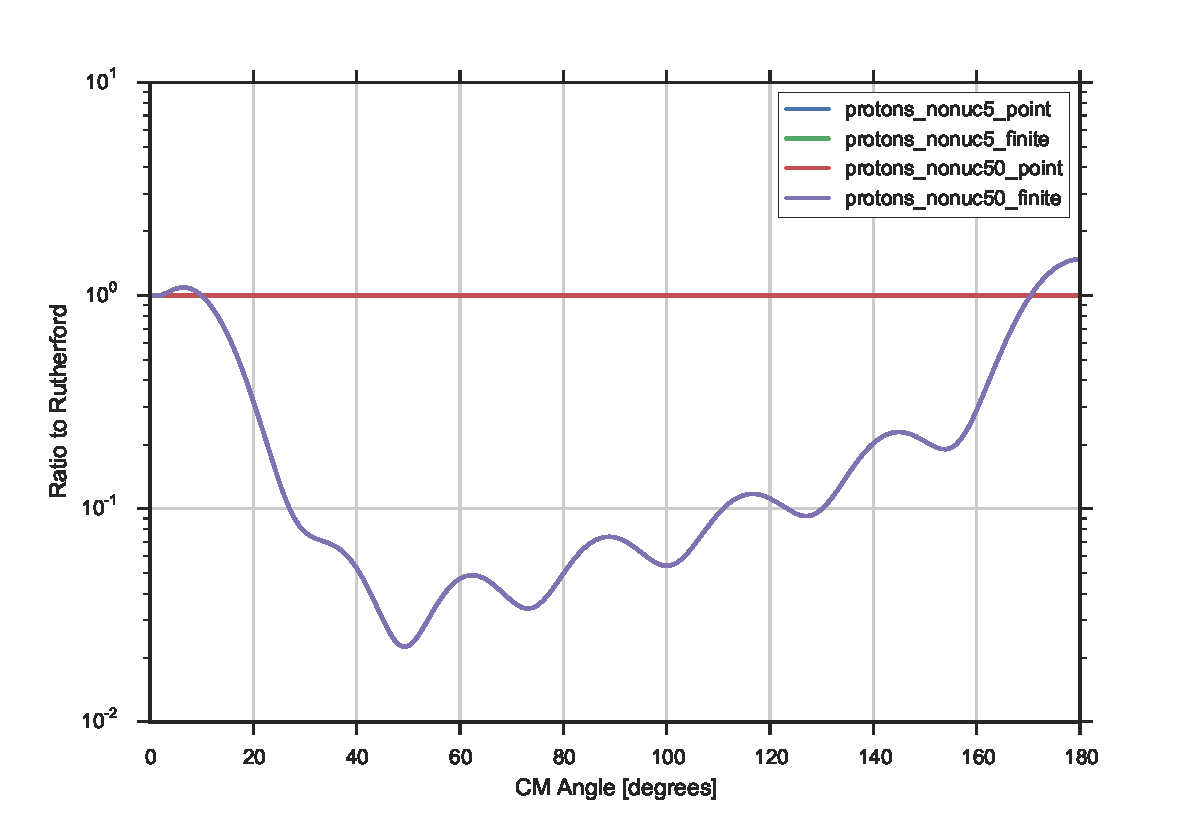
\includegraphics[width=\columnwidth]{{images/protons_nonuc.pdf}}
		\caption{Elastic scattering cross sections for protons on \nuc{100}{Mo} at \SI{5}{MeV} and \SI{50}{MeV} for point-like and finite-radius potentials. This does not include a nuclear potential.}
		\label{fig:protons_nonuc}
	\end{figure}

	\begin{figure}[tb]
		\centering
		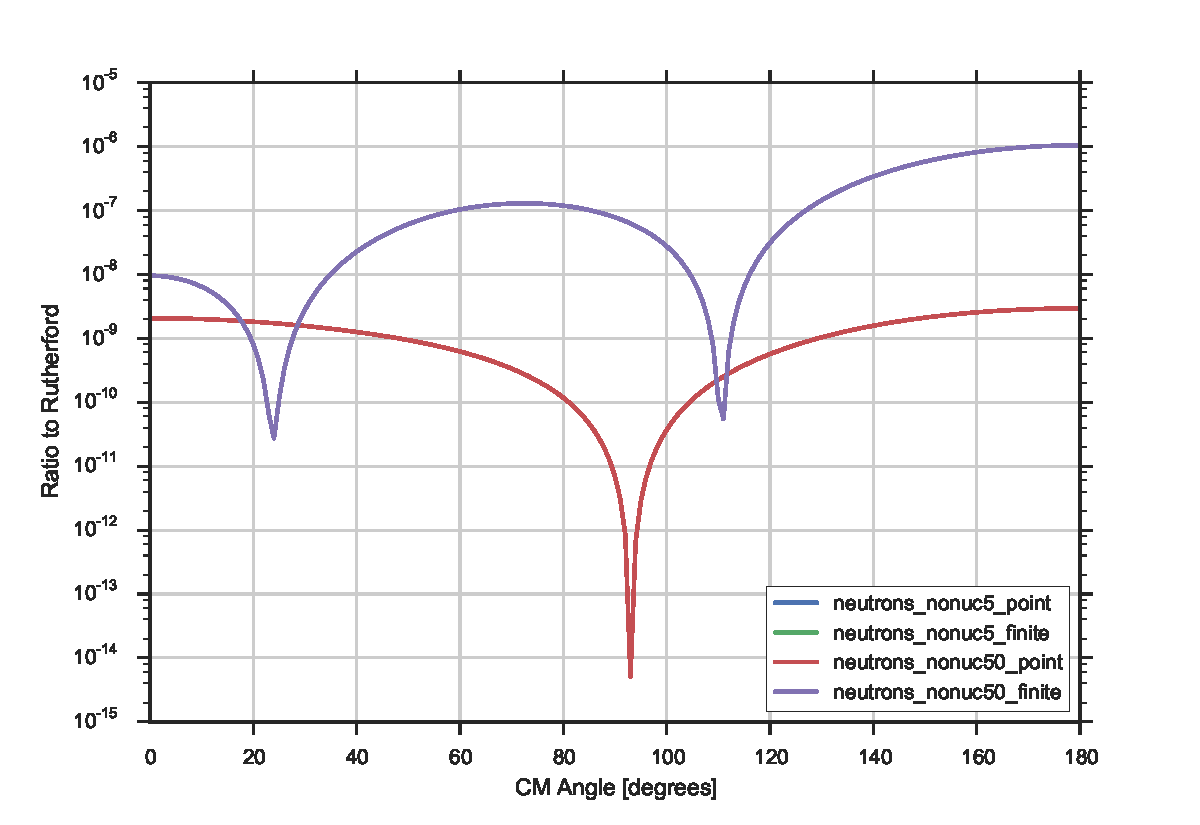
\includegraphics[width=\columnwidth]{{images/neutrons_nonuc.pdf}}
		\caption{Elastic scattering cross sections for neutrons on \nuc{100}{Mo} at \SI{5}{MeV} and \SI{50}{MeV} for point-like and finite-radius potentials. This does not include a nuclear potential.}
		\label{fig:neutrons_nonuc}
	\end{figure}

	\subsection{Nuclear potential}

	Next, we added a nuclear potential. We used a global optical potential of Woods-Saxon shape with parameters from Koning and Delaroche. \cite{Koning2003} We did this for both neutrons and protons. The angular distributions are shown in Fig.~\ref{fig:nuc_all}.

	We can see the following things:
	\begin{enumerate}
		\item For protons at low energy, the scattering cross sections are very close to Rutherford. This is because the low-energy proton does not probe beyond the Coulomb barrier.

		\item As before, the high-energy protons penetrate the Coulomb barrier. This leads to a more complex angular distribution since the proton sees the internal structure of the nucleus.

		\item For both energies, the neutrons probe the nuclear potential. This is because they are not affected by Coulomb repulsion. We also see that there is less scattering at backwards angles for the higher-energy neutrons.
	\end{enumerate}

	\begin{figure}[tb]
		\centering
		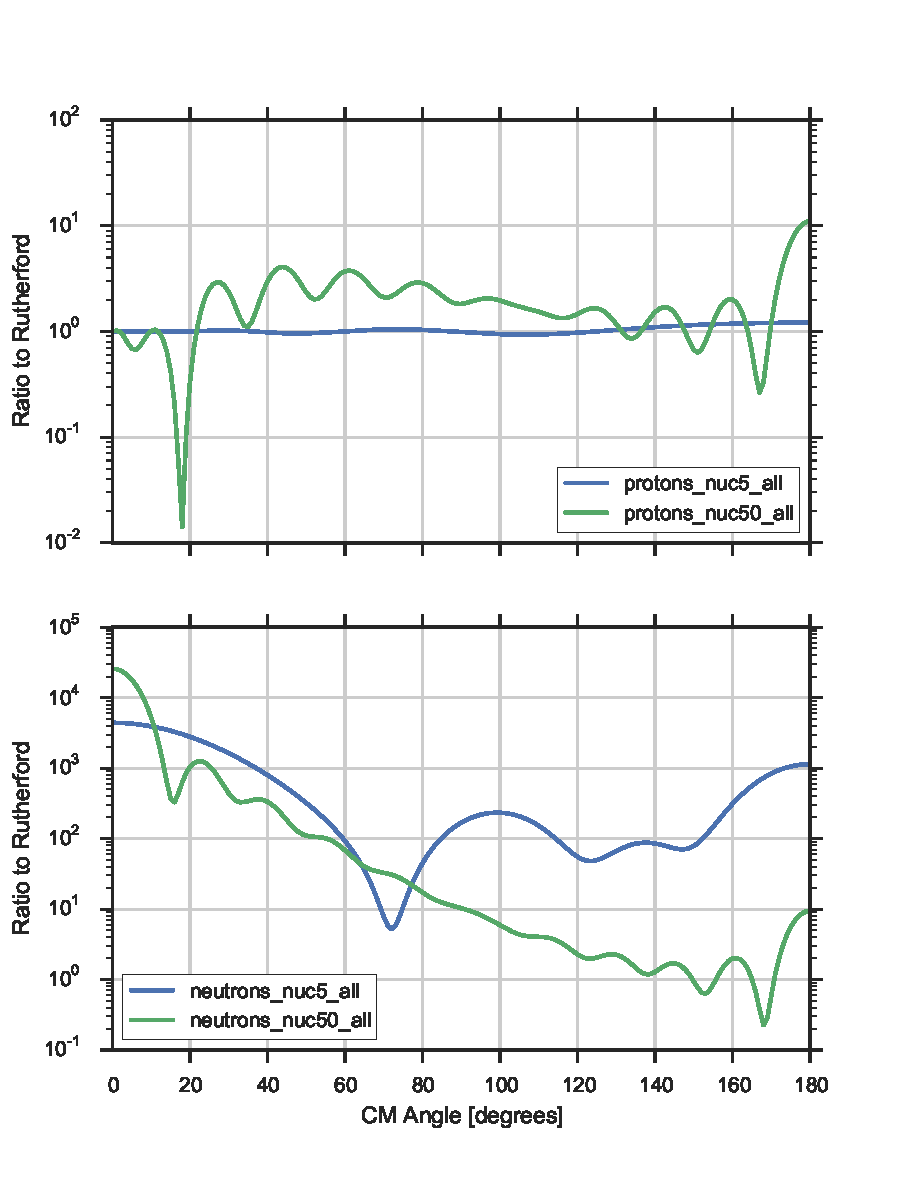
\includegraphics[width=\columnwidth]{{images/nuc_all.pdf}}
		\caption{Elastic scattering cross sections on \nuc{100}{Mo} with a volume nuclear potential for protons (top) and neutrons (bottom) at \SI{5}{MeV} and \SI{50}{MeV}.}
		\label{fig:nuc_all}
	\end{figure}

	\subsection{Contribution of the imaginary part}

	For comparison, we removed the imaginary volume component of the Woods-Saxon nuclear optical potential and examined the behavior of the real part alone. This is shown for both protons and neutrons in Fig.~\ref{fig:nuc_real}. This result looks different from Fig.~\ref{fig:nuc_all} because after removing the imaginary part of the potential, we are no longer accounting for exit channels other than elastic scattering.

	If we compare the $S$ matrices in these two cases, we find that the modulus of the $S$ matrix is 1 for each partial wave in the case of the real potential, as expected. When we add in the imaginary part, the $S$ matrices no longer have a modulus of 1. This indicates that some of the outgoing flux is being absorbed by the imaginary part of the potential. This is shown in Fig~\ref{fig:smat}.

	\begin{figure}[t]
		\centering
		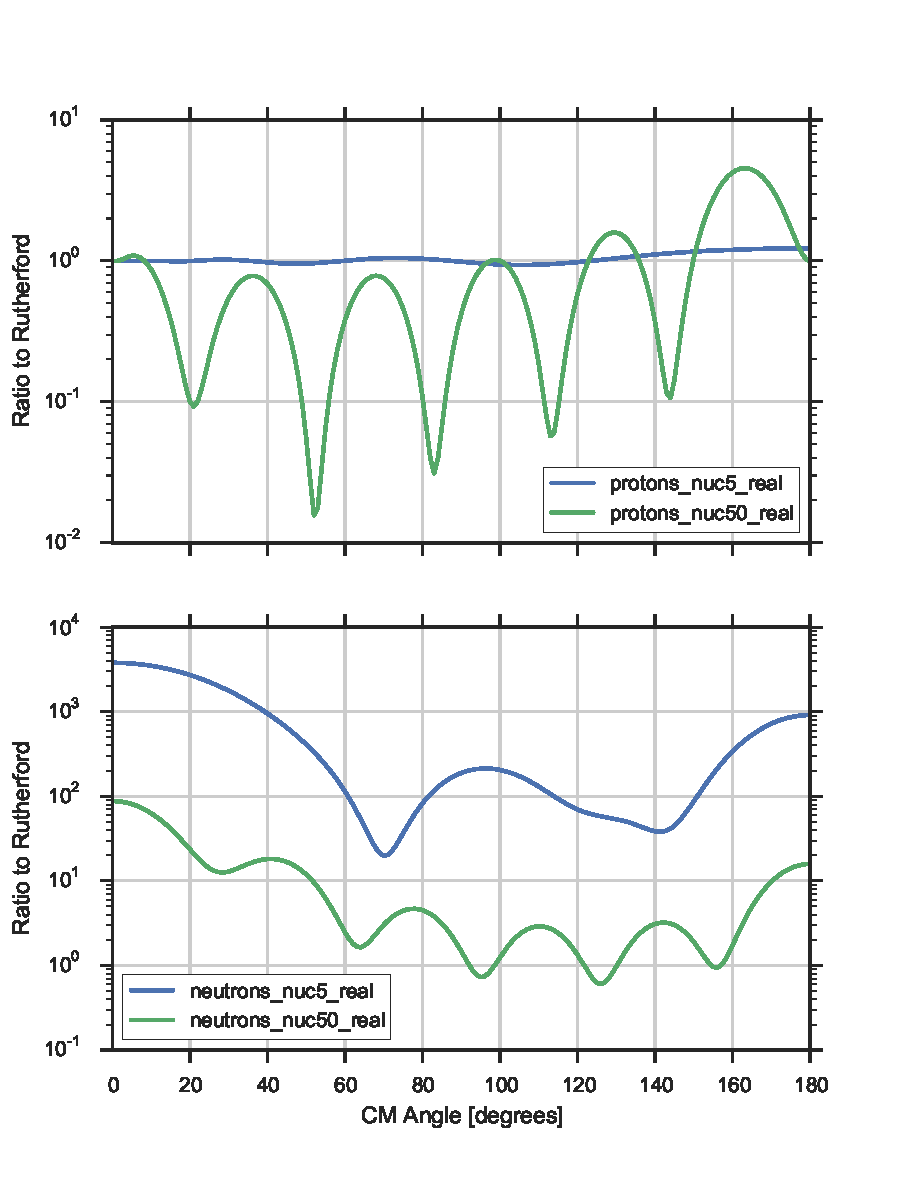
\includegraphics[width=\columnwidth]{{images/nuc_real.pdf}}
		\caption{Elastic scattering cross sections on \nuc{100}{Mo} with only the real component of the volume nuclear potential. This is shown for protons (top) and neutrons (bottom) at \SI{5}{MeV} and \SI{50}{MeV}.}
		\label{fig:nuc_real}
	\end{figure}

	\begin{figure}[tb]
		\centering
		\begin{framed}
		\centering
		\footnotesize
		\begin{verbatim}
			-0.1406733863 -0.9900560582  0  0.5  0.5 : S(L,J,JT)
			-0.9950493561  0.0993819851  1  0.5  0.5 : S(L,J,JT)
			-0.4883262722  0.8726611324  2  1.5  1.5 : S(L,J,JT)
			-0.9950493561  0.0993819851  1  1.5  1.5 : S(L,J,JT)
			-0.4883262722  0.8726611324  2  2.5  2.5 : S(L,J,JT)

			-0.0578241233 -0.4368748881  0  0.5  0.5 : S(L,J,JT)
			-0.4404722371  0.0377326911  1  0.5  0.5 : S(L,J,JT)
			-0.2212677416  0.3878465564  2  1.5  1.5 : S(L,J,JT)
			-0.4404722371  0.0377326911  1  1.5  1.5 : S(L,J,JT)
			-0.2212677416  0.3878465564  2  2.5  2.5 : S(L,J,JT)
		\end{verbatim}
		\end{framed}
		\caption{$S$ matrix elements from \fresco. This is the raw output from the file \texttt{fort.7} for \SI{50}{MeV} protons. The lines above the gap are for the interaction with only the real part, while the lines below the gap are for the interaction with both real and complex parts. It is clear that the moduli of the upper lines are 1.}
		\label{fig:smat}
	\end{figure}

	% \begin{table}[tb]
	% 	\centering
	% 	\begin{ruledtabular}
	% 	\begin{tabular}{c c c c c c}
	% 		  -0.1406733863 & -0.9900560582  &   0  & 0.5  & 0.5 & : S(L,J,JT) \\
	% 		  -0.9950493561 &  0.0993819851  &   1  & 0.5  & 0.5 & : S(L,J,JT) \\
	% 		  -0.4883262722 &  0.8726611324  &   2  & 1.5  & 1.5 & : S(L,J,JT) \\
	% 		  -0.9950493561 &  0.0993819851  &   1  & 1.5  & 1.5 & : S(L,J,JT) \\
	% 		  -0.4883262722 &  0.8726611324  &   2  & 2.5  & 2.5 & : S(L,J,JT) \\
	% 		\colrule
	% 		  -0.0578241233 & -0.4368748881  &   0 &  0.5 &  0.5  & : S(L,J,JT) \\
	% 		  -0.4404722371 &  0.0377326911  &   1 &  0.5 &  0.5  & : S(L,J,JT) \\
	% 		  -0.2212677416 &  0.3878465564  &   2 &  1.5 &  1.5  & : S(L,J,JT) \\
	% 		  -0.4404722371 &  0.0377326911  &   1 &  1.5 &  1.5  & : S(L,J,JT) \\
	% 		  -0.2212677416 &  0.3878465564  &   2 &  2.5 &  2.5  & : S(L,J,JT) \\
	% 	\end{tabular}
	% 	\end{ruledtabular}
	% 	\caption{$S$ matrix elements from \fresco. This is the raw output from the file \texttt{fort.7} for \SI{50}{MeV} protons. The lines above the horizontal rule are for the interaction with only the real part, while the lines below the rule are for the interaction with both real and complex parts. It is clear that the moduli of the upper lines are 1.}
	% 	\label{tab:smat}
	% \end{table}

	\subsection{Increasing the radius}

	Then, we tried increasing the radius parameter in the optical potential and the Coulomb potential to \SI{10}{fm}. We found that it greatly increased the number of oscillations in the graph and increased the total cross section. This is what we expected because making the target larger should increase the cross section. The results are shown in Fig.~\ref{fig:big_r}.

	\begin{figure}[tb]
		\centering
		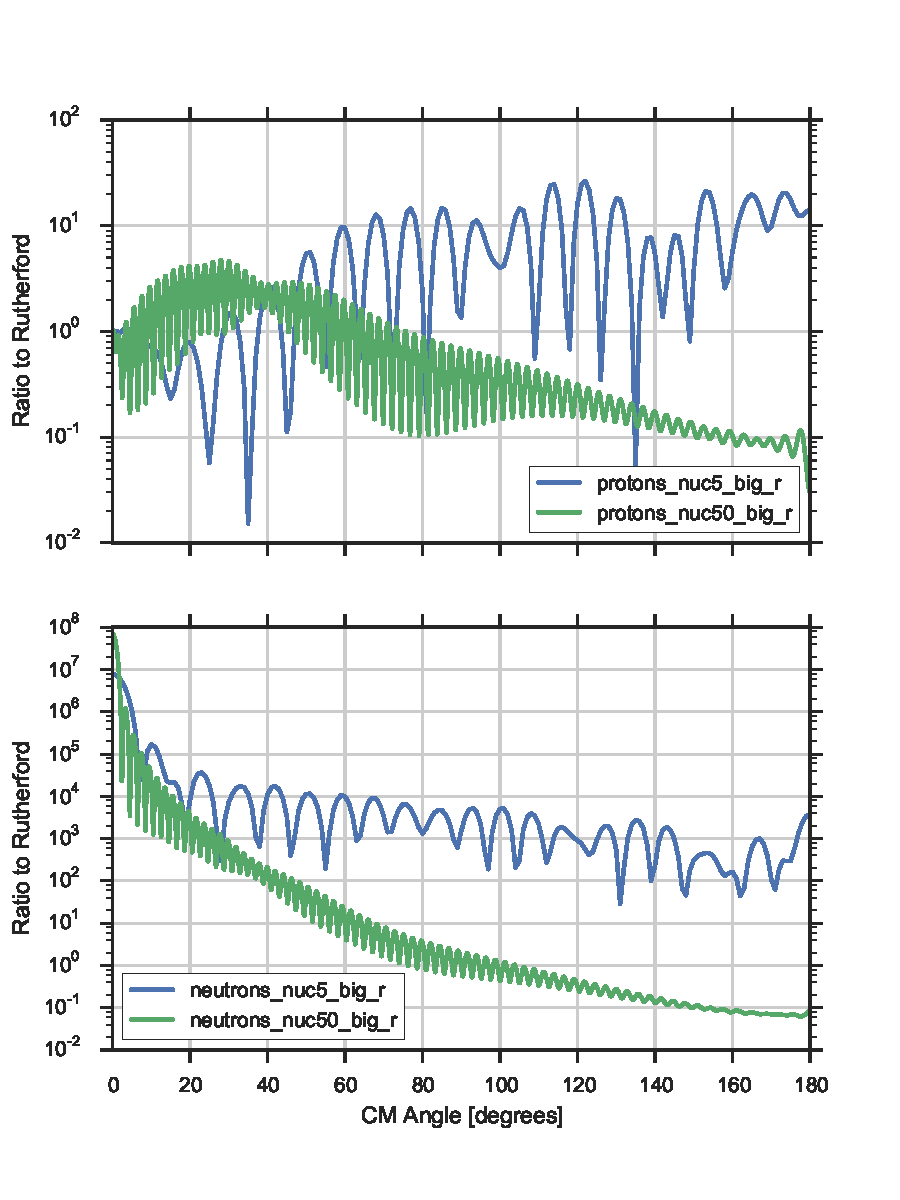
\includegraphics[width=\columnwidth]{{images/big_r.pdf}}
		\caption{Elastic scattering with the radius increased to \SI{10}{fm}.}
		\label{fig:big_r}
	\end{figure}

	\subsection{Total cross-sections}

	Finally, we found the total cross sections for neutron elastic scattering at our two energies. These are shown in Table~\ref{tab:xsec}.

	\begin{table}[h]
		\centering
		\begin{ruledtabular}
		\begin{tabular}{c c c c}
			Energy & Elastic & Absorption & Total \\
			\colrule
			\SI{5}{MeV}  & \SI{4843.87}{mb/sr} & \SI{426.24}{mb/sr} & \SI{5270.11}{mb/sr} \\
			\SI{50}{MeV} & \SI{2597.99}{mb/sr} & \SI{1567.59}{mb/sr} & \SI{4165.57}{mb/sr} \\
		\end{tabular}
		\end{ruledtabular}
		\caption{Neutron scattering cross sections from \fresco.}
		\label{tab:xsec}
	\end{table}


\section{Fitting experimental data}

In this part, we used \sfresco to fit experimental data.  We used data from Sakaguchi et al. \cite{Sakaguchi1982} for elastic scattering of \SI{65}{MeV} protons off of \nuc{100}{Mo}. We performed a variety of fits to this data, and the results from each fit are shown in Table~\ref{tab:params}.

We began by fitting an optical potential with no surface component and no spin-orbit component.  This left six free parameters for the real and imaginary volume potential.  Rather than fitting all six at once, we began by fixing five parameters and only varying the real potential depth. Then we gradually added each remaining parameter one at a time.  Our fit with all six volume potential parameters gave a total $\chi^2/N = 260.324$.  This value, though quite large, is not unexpected because the model does not yet account for a surface imaginary component or a spin-orbit component of the optical potential.  For comparison, we then removed the volume imaginary component and fit the parameters for a surface imaginary component.  This lowered our total $\chi^2/N$ to 149.012.  A comparison of these two fits and the experimental data is shown in Fig.~\ref{fig:fits:a}.

Next we attempted to further improve our fit by adding a spin-orbit component to the real volume and surface imaginary components.  Once again we gradually added parameters to our fit until all nine parameters were included.  This reduced our total $\chi^2/N$ to 52.724.  A comparison of this fit to the surface fit without a spin-orbit component can be seen in Fig.~\ref{fig:fits:b}.

To reduce our $\chi^2/N$ even further, we performed another fit including both volume and surface imaginary components as well as a spin-orbit component in the optical potential.  This resulted in a total of 12 parameters and reduced our total $\chi^2/N$ to 18.833.  A comparison of this fit to the fit with no volume imaginary component is shown in Fig.~\ref{fig:fits:c}.

Finally, we found that the optical parameters obtained by fitting with \sfresco were very sensitive to our initial guesses.  Sakaguchi et al. gave a set of good parameters that they used to fit the data. \cite{Sakaguchi1982}  If we use these parameters as initial guesses and perform another 12-parameter fit in \sfresco, we see that the total $\chi^2/N$ falls to 4.806.  A comparison of this fit to our previous 12-parameter fit is shown in Fig.~\ref{fig:fits:d}.

\begin{figure*}
	\centering
	\subfloat[Volume vs. Surface Potentials]{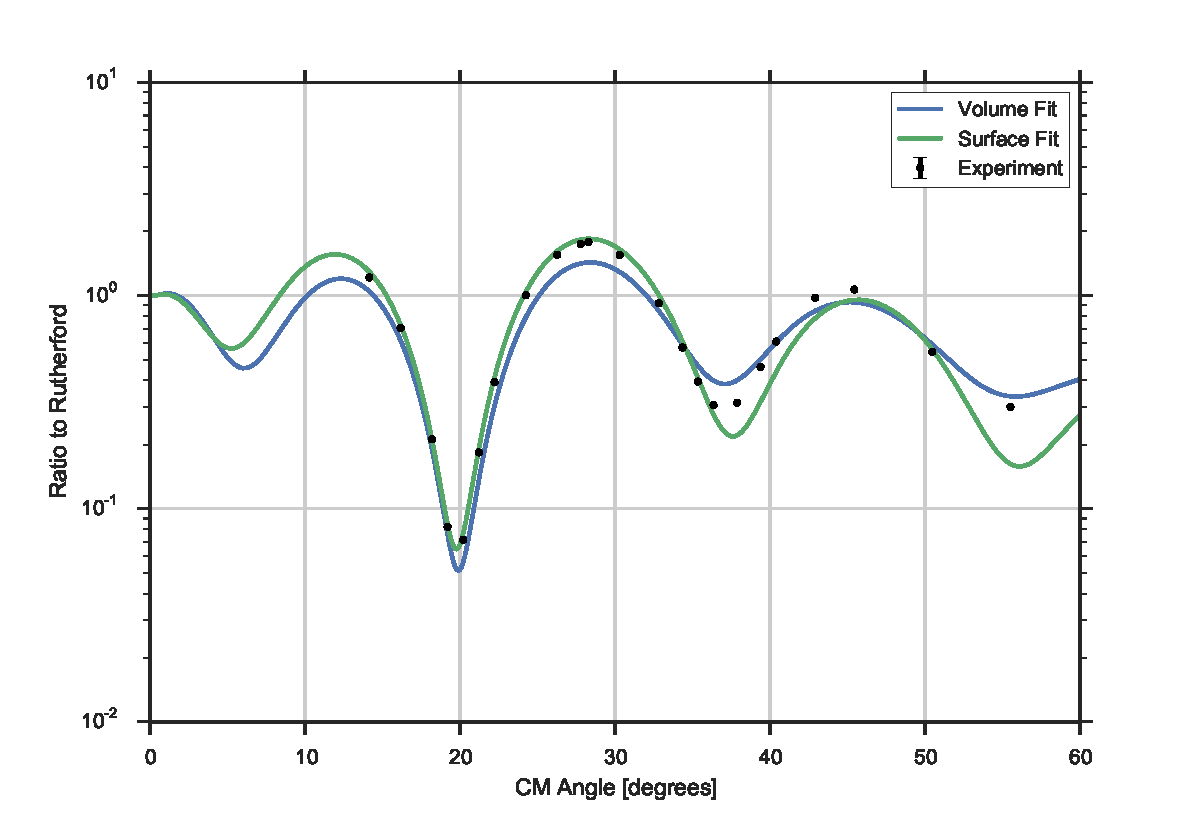
\includegraphics[width=\columnwidth]{images/vol_vs_surf.pdf}\label{fig:fits:a}}
	\subfloat[Surface with and without SO interaction]{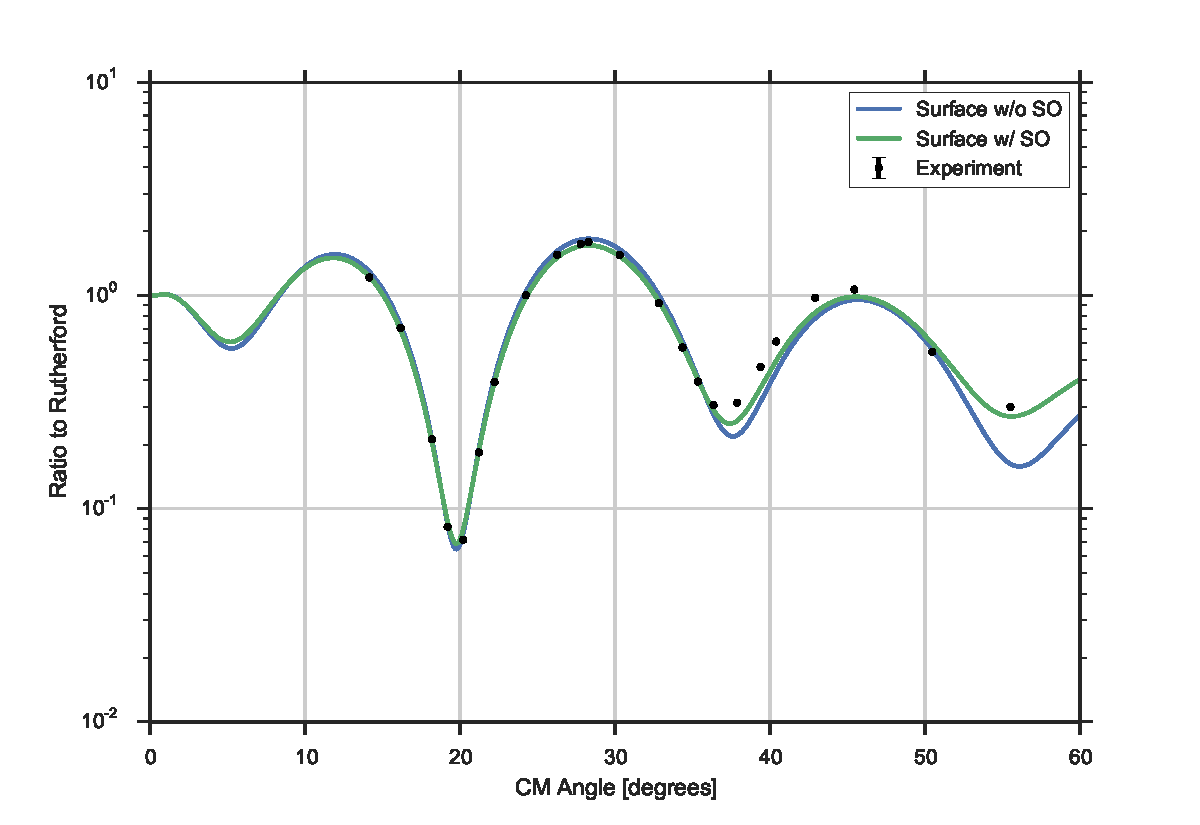
\includegraphics[width=\columnwidth]{images/surf_and_spin.pdf}\label{fig:fits:b}} \\
	\subfloat[Full fit vs. Surface+SO]{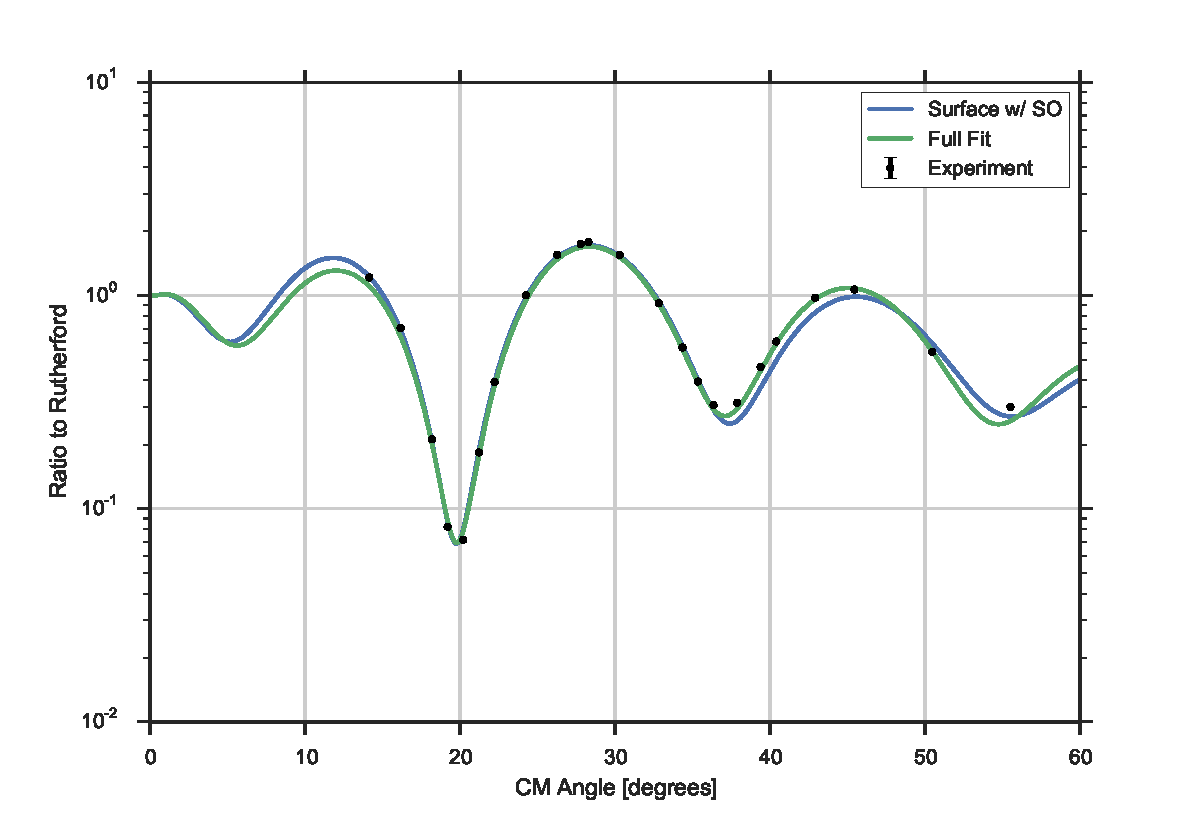
\includegraphics[width=\columnwidth]{images/everything_vs_surfso.pdf}\label{fig:fits:c}} 
	\subfloat[Full fits with different initial conditions]{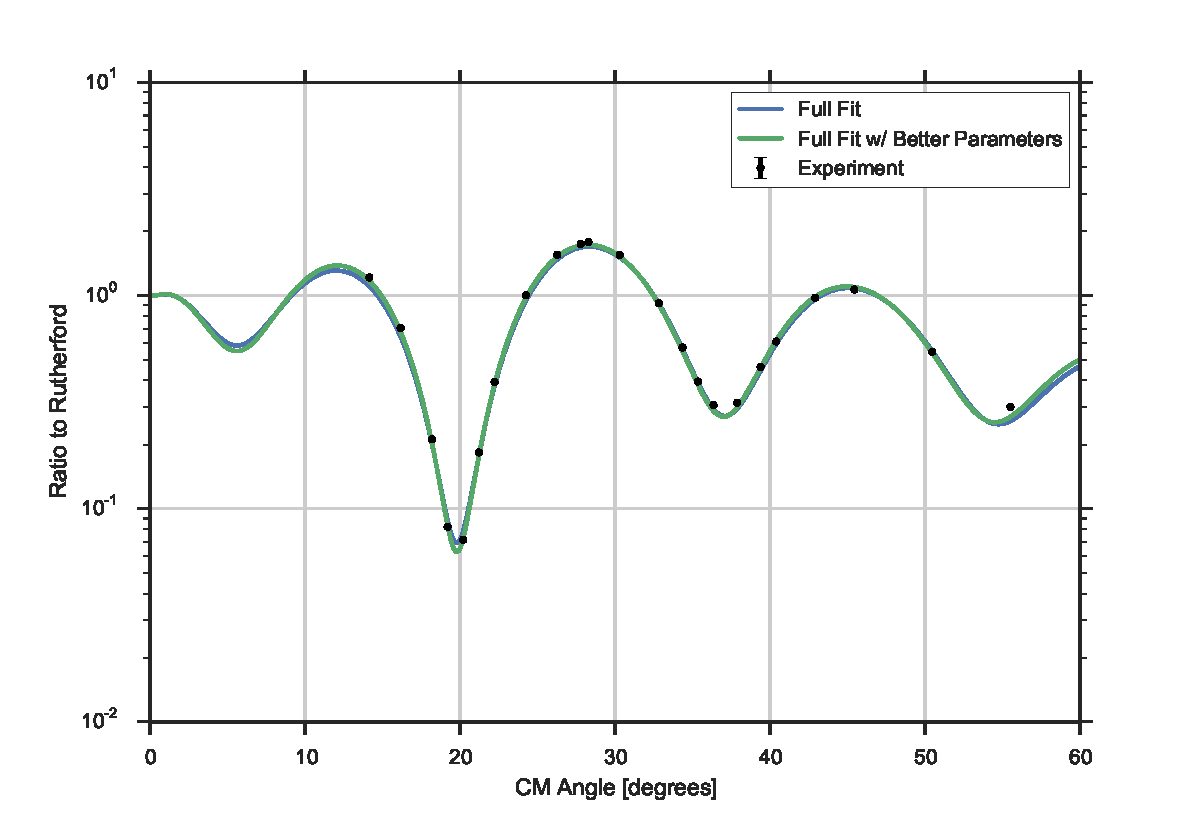
\includegraphics[width=\columnwidth]{images/comp_to_paper.pdf}\label{fig:fits:d}}
	\caption{Angular distributions for scattering of \SI{65}{MeV} protons off of \nuc{100}{Mo}. Black points represent experimental data, and solid curves represent different \sfresco fits to the data. The data points include error bars that are too small to see on the logarithmic scale of this graph. In \protect\subref{fig:fits:a}, a fit with the volume imaginary component is compared to a fit with the surface imaginary component. Graph \protect\subref{fig:fits:b} shows the effect of adding a spin-orbit component to our previous fit that included a surface imaginary component. The next plot \protect\subref{fig:fits:c} adds a volume imaginary component to the surface potential with a spin-orbit component to produce a full fit. The final plot \protect\subref{fig:fits:d} compares two full fits with different sets of initial conditions.}
	\label{fig:fits}
\end{figure*}

\begin{table*}[h]
\begin{ruledtabular}
\begin{tabular}{lllllllllllllr}
Fit          & $V_R$ & $r_R$ & $a_R$ & $W_V$ & $r_V$ & $a_V$ & $W_S$ & $r_S$ & $a_S$ & $V_{SO}$ & $r_{SO}$ & $a_{SO}$ & $\chi^2/N$ \\
\colrule
Volume       & 34.26 & 1.00  & 0.83  & 15.33 & 0.89  & 0.87  &       &       &       &          &          &          & 260.32     \\
Surface      & 37.39 & 1.00  & 0.71  &       &       &       & 5.09  & 1.01  & 0.99  &          &          &          & 149.01     \\
Surface + SO & 36.45 & 1.02  & 0.62  &       &       &       & 6.37  & 1.01  & 0.91  & 5.29     & 1.00     & 0.64     & 52.72      \\
Full         & 38.43 & 0.98  & 0.73  & 6.14  & 0.86  & 0.74  & 5.99  & 1.00  & 0.72  & 6.60     & 0.98     & 0.78     & 18.83      \\
Full 2       & 35.27 & 1.02  & 0.75  & 6.79  & 0.87  & 0.77  & 5.79  & 1.03  & 0.59  & 5.55     & 0.99     & 0.69     & 4.81      
\end{tabular}
\end{ruledtabular}

\caption{Parameters and $\chi^2/N$ values from the various fits. Fits ``Full'' and ``Full 2'' correspond to using all of the parameters, but fit ``Full 2'' uses initial conditions from Sakaguchi et al. \cite{Sakaguchi1982}}
\label{tab:params}

\end{table*}


\bibliography{hw2}

\end{document}